%%%%%%%%%%%%%%%%%%%%%%%%%%%%%%%%%%%%%%%%%%%%%%%%%%%%%%%%%%%%%%%%%%%%%%%%%%
% VoltageAtInductorInCase2
%%%%%%%%%%%%%%%%%%%%%%%%%%%%%%%%%%%%%%%%%%%%%%%%%%%%%%%%%%%%%%%%%%%%%%%%%%

\begin{solutionfigure}[htb]
    \centering
    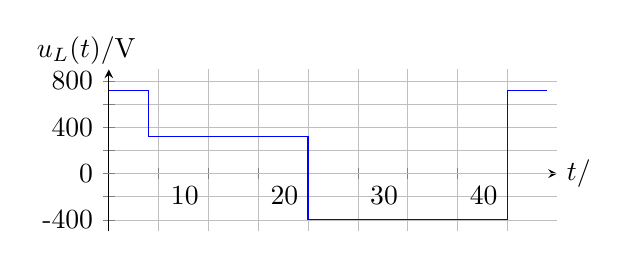
\begin{tikzpicture}
        \begin{axis}[
                domain=0:15,
                % x/y range adjustment
                xmin=0, xmax=45,
                ymin=-500, ymax=900,
                samples=500,
                axis y line=center,
                axis x line=middle,
                extra y ticks=0,
                % Labeltext
                xlabel={$t / \SI{}{\micro\second}$},
                ylabel={$u_\text{L}(t)/\mathrm{V}$},
                % Label adjustment
                x label style={at={(axis description cs:1,0.36)},anchor=west},
                y label style={at={(axis description cs:-.05,.97)},anchor=south},
                width=0.6\textwidth,
                height=0.3\textwidth,,
                % x-Ticks
                xtick={0,5,10,15,20,25,30,35,40},
                xticklabels={0,,10,,20,,30,,40},
                xticklabel style = {yshift=-0.2cm,anchor=east},
                % y-Ticks
                ytick={800,600,400,200,0,-200,-400},
                yticklabels={800,,400,,,,-400},
                % Grid layout
                grid=both,
                grid style={line width=.1pt, draw=gray!10},
                major grid style={line width=.2pt,draw=gray!50},
            ]
            \addplot[color=blue,mark=none,solid] coordinates{
                (0, 720)
                (4, 720)
                (4, 320)
                (20, 320)
                (20, -400)
                (40, -400)
                (40, 720)
                (44, 720)
                };                 
        \end{axis}
    \end{tikzpicture}
    \caption{Voltage at inductor in case 2.}
    \label{fig:VoltageAtInductorInCase2}    
\end{solutionfigure}




